\section*{Átomos multielectrónicos\normalfont{\; \; $\mathcal{H}=H_{\text{cinét}}+H_{\text{pot.nuc.}}+H_{\text{pot.elec.}}+H_{\text{fina}}+H_{\text{hip.fin.}}$}}
\begin{align*}
&\underline{\text{Determinante de Slater}} \; \; \; q_j \equiv \text{coords. gralizadas (espaciales y spin)} \; \; u_\iota(q_j) \equiv \text{fun. onda}\\
&u_\iota (q_j)=u_{n_\iota, l_\iota, m_{l_{\iota}}} (\vec{r}_j)\,\chi_{s_\iota, m_{s_\iota}}(j)\; \; \; N\equiv \text{nº e$^-$}\; \; \; \text{Slater: crea fun.onda ANTISIM}\\
&\text{Nº dets. Slater = nº combinaciones posibles (deg.)\;\;\; Puedes poner entre \{\} los desdobles}\\
&\Psi(q_1,q_2,...,q_N)=\frac{1}{\sqrt{N!}}\cdot \begin{vmatrix} u_\alpha(q_1) & u_\beta(q_1) & ... & u_\omega(q_1) \\ u_\alpha(q_2) & u_\beta(q_2) & ... & u_\omega(q_2) \\ ... & ... & ... & ... \\ u_\alpha(q_N) & \psi_\beta(q_N) & ... & u_\omega(q_N) \end{vmatrix} \\
&\underline{\text{Aprox. Campo Central (C.C.)}}\text{ (potenciales centrales, $H_{e-e}\approx 0$)\;\;\; para e$^-$ i-ésimo:}\\
&\text{lejos núcleo: }U_C^i (r_i)\!=\!-\left[\frac{Ze^2}{4\pi\epsilon_0 r_i}\!-\!\frac{(N-1)e^2}{4\pi\varepsilon_0 r_i}\right]\!\approx\! -\frac{e^2}{4\pi \varepsilon_0}\;\;\;\text{cerca: }U_C^i (r_i)\!=\!-\left[\frac{Ze^2}{4\pi\varepsilon _0 r_i}\right] \\
&E^i=E^i_{n_i,l_i}\;\;\;\text{$l_i\equiv$ fijo: } \uparrow n_i\Rightarrow\;\uparrow E^i_{n_i,l_i} \;\;\;\text{$n_i\equiv$ fijo: } \uparrow l_i\Rightarrow\;\uparrow E^i_{n_i,l_i}\\
&\text{CONFIG. ELECTR.:}\;\; 
\left.\hspace{-9pt}
\begin{array}{l}
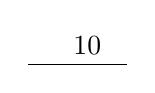
\begin{tikzpicture}
    \draw (0,0) -- (1.25,0);
    \node[above] at (0.75,0) {10};
\end{tikzpicture}\;
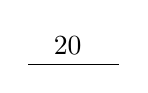
\begin{tikzpicture}
    \draw (1.25,0) -- (2.4,0);
    \node[above] at (01.75,0) {20};
\end{tikzpicture}\hspace{2pt}
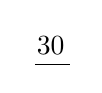
\begin{tikzpicture}
    \draw (2.5,0) -- (2.95,0);
    \node[above] at (2.7,0) {30};
\end{tikzpicture}\hspace{2pt}
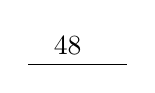
\begin{tikzpicture}
    \draw (3,0) -- (4.25,0);
    \node[above] at (3.5,0) {48};
\end{tikzpicture}\hspace{2pt}
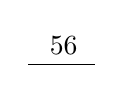
\begin{tikzpicture}
    \draw (4.3,0) -- (5.15,0);
    \node[above] at (4.75,0) {56};
\end{tikzpicture}\hspace{2pt}
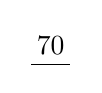
\begin{tikzpicture}
    \draw (5.2,0) -- (5.7,0);
    \node[above] at (5.45,0) {70};
\end{tikzpicture}\hspace{2pt}
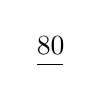
\begin{tikzpicture}
    \draw (5.725,0) -- (6.05,0);
    \node[above] at (5.9,0) {80};
\end{tikzpicture}\hspace{2pt}
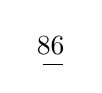
\begin{tikzpicture}
    \draw (6.1,0) -- (6.35,0);
    \node[above] at (6.2,0) {86};
\end{tikzpicture}
\\
1s^2\, 2s^2\, 2p^6\, 3s^2\, 3p^6\, 4s^2\, 3d^{10}\, 4p^6\, 5s^2\, 4d^{10}\, 5p^6\, 6s^2\, 4f^{14} \,5d^{10} \,6p^6  \\[1pt]
\hspace{-5pt}
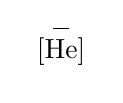
\begin{tikzpicture}
    \draw (0,0) -- (0.2,0);
    \node[below] at (0.1,0) {[He]};
\end{tikzpicture}
\hspace{-2pt}
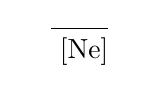
\begin{tikzpicture}
    \draw (0.22,0) -- (0.95,0);
    \node[below] at (0.5,0) {\;\;\;[Ne]};
\end{tikzpicture}\hspace{2pt}
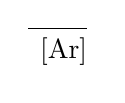
\begin{tikzpicture}
    \draw (1,0) -- (1.75,0);
    \node[below] at (1.45,0) {[Ar]};
\end{tikzpicture}\hspace{2pt}
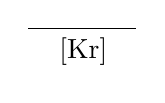
\begin{tikzpicture}
    \draw (1.75,0) -- (3.12,0);
    \node[below] at (2.45,0) {[Kr]};
\end{tikzpicture}\hspace{2pt}
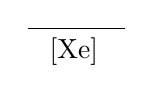
\begin{tikzpicture}
    \draw (3.17,0) -- (4.4,0);
    \node[below] at (3.75,0) {[Xe]};
\end{tikzpicture}\hspace{2pt}
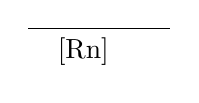
\begin{tikzpicture}
    \draw (4.4,0) -- (6.2,0);
    \node[below] at (5.1,0) {[Rn]};
\end{tikzpicture}
\end{array}
\right.   \\
&\text{Configuración fundamental: aquella que minimice $E$}\\
&\text{Deg: subcapa }nl: g_{nl}=2(2l+1)\;\;\;\;\; \text{capa }n:g_{n}=\Sigma_{l=0}^{n-1}g_{nl}=2n^{2}\\
&\text{Deg. de equiv.: dada config., nº est. posibles con misma E: }g_i=
\begin{matrix}
\binom{2(2 l_i +1)}{\chi_i}, 
\end{matrix}
\text{ donde ...}\\
&\chi_i\text{ es el nº de e$^-$ en la misma subcapa $l_i$. La deg. total de equiv.: }G=\Pi_i g_i.\\
&\text{Incluimos }H_{e-e}, H_{\text{fina}}. \text{ Si $H_{e-e}\!\!>\!\!>\!H_{\text{fina}}\!\rightarrow\!$ ACOP. $L$-$S$, $H_{\text{fina}}\!>\!\!>\!H_{e-e}\rightarrow$ ACOP. $J$-$J$}\\
&\underline{\text{ACOP. L-S (RUSSEL-SAUNDERS)}}\;\;\;\text{$\vec{l}_i, \vec{s}_i$ NO conmutan con $H$; $\vec{L}, \vec{S}$ SÍ }\\
&\text{Términos espectrales: } ^{2S+1}L  \xrightarrow[H_{\text{fina}}]{\text{incluyo}}\text{niveles espectrales: }^{2S+1}L_J\;\; \vec{J}\text{ conserv, }\vec{L},\vec{S} \text{ NO}\\
&\text{deg. térm.: }(2L+1)(2S+1)\;\;\;\;\;\;\;\text{deg. nivel: }(2J+1)\;\;\; \;\;\;\;\text{deg. se pone entre [ ]} \\
&\scalebox{0.8}{$1!\;  e^- \text{ por subcapa: $e^-$ no equiv.}\rightarrow\text{térms: con}\oplus\;\;\;\;\;\text{varios $e^-$ en misma capa: $e^-$ equivs.}\rightarrow$\text{térms: con tabla}}\\
&\scalebox{0.8}{
\text{Térm. esp.: tablas \textit{a)} (solo 2 $e^-$) o \textit{b)} (varios). Simpre cumple Pauli: NO ($a\uparrow, a\uparrow$) TACHA si $\nexists$ conf. posib.}}\\
&\scalebox{0.8}{\text{NO repitas:($i\uparrow, j\uparrow$)=($j\uparrow, i\uparrow$)\;\;\ Comprueba deg. equiv. coincide. \;\;\ Desdoble $n l^k=nl^{g_{\scalebox{0.8}{nl}}-k}$ (orden inverso)}}\\
&\scalebox{0.8}{\text{Si $nl\,n'l' (n\neq n')$: find microest. separately y combine  con $\oplus$. Puede $\exists$ ($i\uparrow,i\uparrow,j\uparrow$) si $i$'s de distintos n.}}\\
&\scalebox{0.8}{\text{a) 1ª fila (col): $m_{l_{1(2)}},$ 2ª fila(col): $m_{s_{1(2)}}.$ Celdas: $(m_{l_1}\!\!+\!\!m_{l_2}, m_{s_1}\!\!+\!\!m_{s_2})$. Take máx $L,S$ y run $\{M_L,M_S\}$}}\\
&\scalebox{0.8}{\text{b) Posibles $M_S\!:$1ª fil, $M_L\!:$1ª col. Celdas: posibles ($m_{l_1} m_{s_1},...,m_{l_n}m_{s_n}$),, sumen 1ª fil y col. Take y run.}}\\
&\scalebox{0.8}{\text{solo necesario 1/4 tabla b) por simetría (inversión spin y/o ·-1) While run no posible tick: corresp. al último L,}}\\
&\scalebox{0.8}{\text{pero siguiente S. Si $\nexists$ sig. S, microestado doble, indica (2) delante, deg. ·2. \;\;\; Est. fund.: aquel que maximiza:}}\\
&\scalebox{0.8}{\text{1º $M_S$, 2º $M_L$ (estruct. fina según semillenado). Write posibles estados en capa $l$, cumple rules y Pauli.}}
\end{align*} 
\vspace{-10pt}
\begin{align*}
&\text{HUND: 1. Térms. $\uparrow$S\,\;$\downarrow$E \;\;2. S fijo, $\uparrow$L\,\;$\downarrow$E \;\;\; 3.Subcapa $\displaystyle \scalebox{0.7}{$\stackrel{>}{<}$}$\ 
semi-llena $\displaystyle \scalebox{0.8}{$\stackrel{\downarrow\; \text{E}\;: \uparrow J\text{(inverso)}}{\downarrow \text{E}: \downarrow J\text{(normal)}}$}$}
\\
\vspace{-7pt}
&\scalebox{0.8}{\text{Si llenado semilleno: $\nexists$ desdoblamiento, todos niveles misma energía p.q. $\tilde{A}$=0 si subcapa semillena.}}
\end{align*}
\begin{align*}
    &\text{REGLA Landé ($H_{\text{fin,S-O}}$)}: \Delta E_{S\text{-}O}\!=\!\tilde{A}(\gamma LS)\,\frac{\hbar^2}{2} [J(J\!+\!1)\!-\!L(L\!+\!1)\!-\!S(S\!+\!1)]\left.\hspace{-1pt}
\begin{array}{c}
\tilde{A}\equiv\text{cte}\\
\text{acop. S-O}
\end{array}
\right.\\
&\text{Indica distinta $\tilde{A}$ en función de $L,S$. Valora $\tilde{A}(\gamma,L,S)$ positiva o negativa según Hund.}\\
&\underline{\text{ACOPLO J-J}} \;\;\vec{l}_i, \vec{s}_i \text{ NO conmutan con H}, \vec{j}_i \text{ SÍ}\;\;\; \nexists \text{ reglas as Hund}\rightarrow
\left.\hspace{-1pt}
\begin{array}{c}
\text{asemeja deg L-S}\\
+\text{ mín cuts}
\end{array}
\right.
&\text{Términos espetrales: }(j_1,...,j_n)\xrightarrow{\text{incluyendo } H_{e\text{-}e}} (j_1,...,j_n)_J\;\;\;\; \vec{J}\text{ conservado, $\vec{{j}}_i$ NO}\\
&\text{deg. térm.: si e$^-$ equivs Y }j_1=j_2 \Rightarrow \binom{2j\!+\!1}{N},\;\; \text{else: }\Pi_{i}(2j_i\!+\!1)\;\;\;\text{deg. nivel: }(2J\!+\!1)\\
&\text{e$^-$ no equiv: $j_i$ con $\oplus$ y join en (,)}\;\;\;\;\; \text{e$^-$ equiv: tabla j-j) y proced. similar}\\
&\text{para varios e$^-$, hago primero 2, y acoplo de 1 en 1 con $\oplus$ y asegurando Pauli}
&\underline{\text{Estructura Hiperfina}} \;\; \vec{F}=\vec{I}+\vec{J}\;\;\;\;\;\Delta E_{\text{h.f.}}= \frac{\mathcal{A}\hbar^2}{2}[F(F+1)-J(J+1)-I(I+1)]\\
&\text{\underline{Otros}: Paridad ($\pi$): $(-1)^{\sum_i l_i}$\;\;
$\left.\hspace{-5pt}
\begin{array}{c}
+ \;\; \text{par}\\
-\;\;\text{impar}
\end{array}
\right.$\;\;\;
Indica con ' distintas  $\mathcal{A}$ en función de $J$}
\end{align*}